\fancyhead[RO,LE]{\thepage}
\fancyfoot{} 
\chapter{An Efficient Parallel Algorithm}
\label{chapter:parallel}

In the previous chapter, I describe a sequential algorithm for updating the level set field according to a sparse and dynamic active computational domain that is coherent in space and time. In this chapter I map this sequential algorithm onto massively parallel hardware.

Parallelizing the sequential algorithm from the previous chapter is challenging because the algorithm assumes the availability of mathematical sets (i.e. collections that are guaranteed not to contain duplicate elements) in the progamming model. The following scenario highlights the difficulty of implementing the functionality of mathematical sets on massively parallel hardware. Suppose two threads want to simultaneously add the same element to a set. Suppose this element does not currently exist in the set. Without proper synchronization, it will appear to both threads as though the element does not exist in the set. In this case both threads will decide that they must add the same element to the set. After both threads add the same element to the set, the element will then appear in the set twice. Therefore the set will fail to exclude duplicate elements. Solving this problem with per-thread synchronization mechanisms like locks and atomic memory operations scales poorly on massively parallel hardware.

\section{Algorithm Overview}

For reasons described in Chapter \ref{chapter:background}, I prefer parallel algorithms that are both work-efficient and step-efficient. Since the sequential algorithm in the previous chapter has $O(n)$ work-complexity, I would prefer the parallelized version of this algorithm to have work-complexity of at most $O(n)$ and step-complexity of at most $O(\log n)$. This upper bound on work-complexity and step-complexity motivates the parallel algorithm described in this chapter.

\begin{samepage}
A high level overview of my parallel algorithm is as follows:

\begin{enumerate}

    \item Initialize the level set field and generate a dense list of active coordinates.

    \item Update the level set field at all active coordinates.

    \item Generate new active coordinates. During this step generating duplicate active coordinates is permitted.

    \item Remove all duplicate active coordinates generated in (3).

    \item Compact all the unique new active coordinates from (4) into a new dense list.

    \item If there are no active coordinates in the new dense list, the segmentation has globally converged. Otherwise go to (2).

\end{enumerate}
\end{samepage}

%-------------------------------------------------------------------------
\section{Assumptions}
\label{subsec:assumptions}

I assume $ \phi $ is 3D and the voxels in $ \phi $ are 6-connected. Therefore it is guaranteed that for all voxels $ \boldx \in \domainphi $, the set $ \nx $ contains at most seven elements: the 6-connected neighbors of $ \boldx $ and $ \boldx $ itself. I define the set $ E = \leftcbracket \leftbracket 0,0,0 \rightbracket , \leftbracket \pm 1,0,0 \rightbracket , \leftbracket 0,\pm 1,0 \rightbracket , \leftbracket 0,0,\pm 1 \rightbracket \rightcbracket $ as the set of offset vectors from a voxel to its 6-connected neighbors.

%-------------------------------------------------------------------------
\section{Data Structures and Notation}
\label{subsec:dataStructuresAndNotation}

My algorithm requires three 3D buffers: $\phiwrite$ and $\phiread$ to store the current and previous level set field respectively; and $U$ to use as a scratchpad. My algorithm also requires eight 1D buffers: $V$ to store the current dense list of active coordinates; and $B^{ \leftbracket 0,0,0 \rightbracket }$, $B^{ \leftbracket \pm 1,0,0 \rightbracket }$, $B^{ \leftbracket 0, \pm 1,0 \rightbracket }$, and $B^{ \leftbracket 0,0, \pm 1 \rightbracket }$ to use as auxiliary buffers when generating new active coordinates. The size of each buffer is equal to the size of the entire level set field. All buffers are initially filled with null values.

I use a subscript notation to refer to individual buffer elements. For example $V_i$ refers to the $i^{th}$ element of $V$; $V_{j \ldots k }$ refers to the range of elements in $V$ from $V_j$ to $V_k$; and $U_{\boldx}$ refers to the element of $U$ with the 3D coordinates $\boldx$.

%We use $V$ to store the current set of active coordinates. We use $\phiread$ and $\phiwrite$ to read from and write to the level set field in a double-buffered fashion. We use $ B^{ \leftbracket 0,0,0 \rightbracket }$, $B^{ \leftbracket 0,0, \pm 1 \rightbracket }$, $B^{ \leftbracket 0, \pm 1,0 \rightbracket }$, and $B^{ \leftbracket \pm 1,0,0 \rightbracket }$ as auxiliary buffers to store intermediate output as we're generating new active coordinates. Finally we use $U$ as a scratchpad buffer. All buffers are initially filled with null values.

%-------------------------------------------------------------------------
\section{Initialization}
\label{subsec:initialization}


\begin{Listing}[t]
    \caption{Initializing the level set field to the signed and clamped distance transform relative to a user-specified seed sphere with the center \textbf{c} and the radius \textit{r}. \label{pseudo:1} }
    \begin{algorithmic}[1]
        \FORALL { coordinates $\boldx \in \domainphi$ in parallel } 
            \STATE { $ \phiread_{\boldx} \gets \mbox{clamp} \leftbracket \| \boldx - \mathbf{c} \| - r \rightbracket $  }
            \STATE { $ \phiwrite_{\boldx} \gets \mbox{clamp} \leftbracket \| \boldx - \mathbf{c} \| - r \rightbracket $  }
        \ENDFOR
    \end{algorithmic}
\end{Listing}


\begin{Listing}[t]
    \caption{Initializing the list of active coordinates. The spatial derivative of the level set field is tested on line 5. \label{pseudo:2} }
    \begin{algorithmic}[1]
        \FORALL { coordinates $\boldx \in \domainphi$ in parallel }
            \STATE { $ g \gets \mbox{false} $ }
            \FORALL { coordinates $\boldn \in \nx$ }
                \IF { \textbf{not } $ g $ }
                    \IF { $ \phiread_{\boldx} \neq \phiread_{\boldn} $  }
                        \STATE { $ g \gets \mbox{true} $ }
                    \ENDIF    
                \ENDIF
            \ENDFOR
            \IF { $ g $ }
                \STATE { $ U_{\boldx} \gets \boldx $  }
            \ENDIF           
        \ENDFOR
        \STATE { $ V \gets \mbox{\textbf{compact}} \leftbracket U \rightbracket $  }
    \end{algorithmic}
\end{Listing}


I initialize in parallel every coordinate in $\phiread$ and $\phiwrite$ according to a user-specified seed region as shown in Listing~\ref{pseudo:1}. For more details on this initialization step I refer the reader to Lefohn et al.~\cite{Lefohn-2004}.

I then generate a densely packed buffer of active coordinates $V$ based on the contents of $\phiread$ as shown in Listing~\ref{pseudo:2}. I test every coordinate of $\phiread$ in parallel to determine which ones are active. If a coordinate is deemed active according to Equation~\ref{eq:active}, I write that coordinate to my 3D scratchpad $U$ using the coordinate itself as the 3D array index. I compact $U$ in parallel to produce $V$. I set the initial size of the active computational domain $n$ to be the number of coordinates that were compacted into $V$. I note that since $U$ contains either a unique value or null at all coordinates, it is guaranteed that there are no duplicate coordinates in $V_{0 \ldots n}$. At this point my algorithm has been fully initialized. I avoid traversing the entire level set field for the remainder of my algorithm.


%*******************************************************************************
% FIGURE 2
%\begin{figure}[t]
%\centering
%\includegraphics[width=6.0in]{figs/fig2.png}
%\caption{Initializing our list of active coordinates in parallel. We initialize in parallel a scratchpad buffer with active coordinates using the coordinates themselves as array indices. We then interpret the scratchpad buffer as one-dimensional and compact it in parallel to produce a densely packed buffer of active coordinates.}
%\label{fig:2}
%\end{figure}
%*******************************************************************************


%-------------------------------------------------------------------------
\section{Updating the Level Set Field}
\label{subsec:updatingTheLevelSetField}


\begin{Listing}[t]
    \caption{Updating the level set field according to Equation~\ref{eq:levelseteq} and clearing the scratchpad at all active coordinates. $n$ is the current size of the active computational domain. \label{pseudo:3} }
    \begin{algorithmic}[1]
        \FORALL { coordinates $\boldv \in V_{0 \ldots n}$ in parallel }
            \STATE { $ \phiwrite_{\boldv} \gets \phiread_{\boldv} + \Delta t F \leftbracket \boldv , t \rightbracket \ \leftvbracket \nabla \phiread_{\boldv} \rightvbracket $ }        
            \STATE { $ U_{\boldv} \gets \mbox{null} $  }                
        \ENDFOR
        \STATE { $ \mbox{\textbf{swap}} \leftbracket \phiread, \phiwrite \rightbracket $  }        
    \end{algorithmic}
\end{Listing}



During each iteration I update $\phiwrite$ and clear $U$ at all active coordinates as shown in Listing~\ref{pseudo:3}. This is guaranteed to completely clear $U$ because the only non-null values in $U$ are at active coordinates, each of which was previously compacted into $V$. At this point I am finished updating the level set field for this iteration, so I swap references to $\phiread$ and $\phiwrite$.

It is important to note that for a given iteration $t$, it is actually the case that $\phiwrite = \phi \leftbracket t - 2 \Delta t \rightbracket $ and $ \phiread = \phi \leftbracket t - \Delta t \rightbracket $ prior to writing new level set values into $\phiwrite$. Since I do not update every voxel at every iteration, I must ensure that the old values from $t - 2 \Delta t$ are allowed to remain in $ \phiwrite $ only if they have not changed from iteration $t - 2 \Delta t$ to iteration $t - \Delta t$. Otherwise I must ensure that these values are updated. Fortunately if $\phixtmtdt \neq \phixtmdt $, then Equation \ref{eq:active} guarantees $ \boldx \in A \leftbracket t \rightbracket $ and a new level set value that depends only on $ \phiread = \phi \leftbracket t - \Delta t \rightbracket $ will be written into $ \phiwrite $ at $ \boldx $.



%-------------------------------------------------------------------------
\section{Generating New Active Coordinates}
\label{subsec:generatingNewActiveCoordinates}


%*******************************************************************************
% FIGURE 3
\begin{figure}[t]
\centering
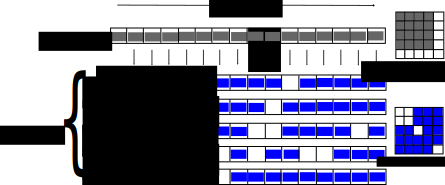
\includegraphics[width=6.0in]{figures/NewActive.pdf}
\caption{Generating new active coordinates. There may be duplicate coordinates in the auxiliary buffers when taken collectively. All duplicate coordinates must subsequently be removed (see Figure~\ref{fig:4}).}
\label{fig:3}
\end{figure}
%*******************************************************************************


%*******************************************************************************
\begin{Listing}[t]
    \caption{Generating new active coordinates. The temporal and spatial derivatives of the level set field are tested on line 5. $n$ is the current size of the active computational domain. \label{pseudo:4} }
    \begin{algorithmic}[1]
        \FOR { $h \gets 0$ to $n$ in parallel }
            \STATE { $\boldv \gets V_h$ } 
            \STATE { $g \gets \mbox{false}$ }
            \FORALL { coordinates $\boldn \in \nv$ }
                \IF { $ \phiread_{\boldn} \neq \phiwrite_{\boldn} $ \textbf{ and } $ \phiread_{\boldn} \neq \phiread_{\boldv} $ }
                    \STATE { $g \gets \mbox{true}$ }
                    \STATE { $\mathbf{e} \gets \boldn - \boldv$ }
                    \STATE { $B^{\mathbf{e}}_{h} \gets \boldn $ }
                \ENDIF
            \ENDFOR
            \IF { $g$ }
                \STATE { $B^{ \leftbracket 0,0,0 \rightbracket }_{h} \gets \boldv $ }
            \ENDIF                    
        \ENDFOR
    \end{algorithmic}
\end{Listing}
%*******************************************************************************


I traverse my current list of active coordinates in parallel and test for new active coordinates according to Equation~\ref{eq:active}. I describe this process in Listing~\ref{pseudo:4} and Figure~\ref{fig:3}. I test $ { \varsigma }_{1} $ and $ { \varsigma }_{2} $ for the next iteration by examining $ \phiread = \phi \leftbracket t \rightbracket $ and $ \phiwrite = \phi \leftbracket t - \Delta t \rightbracket$. I note that at the end of this step, the seven auxiliary buffers may contain duplicate coordinates when taken collectively. This is because each thread tests a local neighborhood of coordinates and some coordinates may be tested repeatedly by different threads. For example some thread $p$ may deem a coordinate $\mathbf{r}$ to be active. For the thread $p$ suppose that $\mathbf{r}-\mathbf{v}_p = \leftbracket 0,0,1 \rightbracket$ and therefore thread $p$ writes $\mathbf{r}$ to the auxiliary buffer $B^{ \leftbracket 0,0,1 \rightbracket }$. Some different thread $q$ may also deem the same coordinate $\mathbf{r}$ to be active. For the thread $q$ suppose that $\mathbf{r} - \mathbf{v}_q = \leftbracket 1,0,0 \rightbracket $ and therefore thread $q$ writes $\mathbf{r}$ to the auxiliary buffer $B^{ \leftbracket 1,0,0 \rightbracket }$. In this case $\mathbf{r}$ appears in both $B^{ \leftbracket 0,0,1 \rightbracket }$ and $B^{ \leftbracket 1,0,0 \rightbracket }$.


I also note that since each new active coordinate is the 6-connected neighbor of some old active coordinate, and all 6-connected neighbors of all old active coordinates are tested by at least one thread, it is guaranteed that all new active coordinates are contained in at least one of the seven auxiliary buffers.


%-------------------------------------------------------------------------
\section{Removing Duplicate Active Coordinates}
\label{subsec:removingDuplicateActiveCoordinates}


%*******************************************************************************
% FIGURE 4
\begin{figure}[t]
\centering
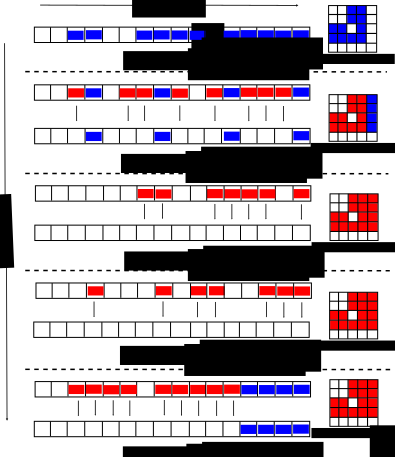
\includegraphics[width=6.0in]{figures/RemoveDuplicates-Alt.pdf}
\caption{Removing duplicate coordinates from the auxiliary buffers in parallel without sorting. Coordinates that have not been previously tagged in the scratchpad buffer are shown in blue. Coordinates that have been previously tagged in the scratchpad buffer are shown in red, and are removed from their containing auxiliary buffer. This process is free of race conditions because each step examines one auxiliary buffer and there are no duplicate coordinates within each auxiliary buffer.}
\label{fig:4}
\end{figure}
%*******************************************************************************

%*******************************************************************************
\begin{Listing}[t]
    \caption{Generating a new dense list of unique active coordinates without sorting the auxiliary buffers. $n$ is the current size of the active computational domain. \label{pseudo:5} }
    \begin{algorithmic}[1]
        \STATE { $ E' \gets E - \leftcbracket \leftbracket 0,0,0 \rightbracket , \leftbracket 0,0,1 \rightbracket \rightcbracket $ }
        \FORALL { coordinates $\mathbf{b} \in B^{ \leftbracket 0,0,0 \rightbracket }_{0 \ldots n}$ in parallel }
            \IF { $ \mathbf{b} \neq \mbox{null}$ }
                \STATE { $ U_{\mathbf{b}} \gets \mbox{tagged}$ }
            \ENDIF
        \ENDFOR                        
        \FORALL { offset vectors $\mathbf{e} \in E' $ } 
            \FOR { $h \gets 0$ to $n$ in parallel }
                \STATE { $\mathbf{b} \gets B^{\mathbf{e}}_{h}$ }            
                \IF { $ \mathbf{b} \neq \mbox{null}$ }
                    \IF { $ U_{\mathbf{b}} = \mbox{tagged} $ }
                        \STATE { $B^{\mathbf{e}}_{h} \gets \mbox{null}$ }
                    \ELSE
                        \STATE { $U_{\mathbf{b}} \gets \mbox{tagged} $ }
                    \ENDIF                                            
                \ENDIF
            \ENDFOR
        \ENDFOR
        \FOR { $h \gets 0$ to $n$ in parallel }
            \STATE { $\mathbf{b} \gets B^{ \leftbracket 0,0,1 \rightbracket }_{h} $ }       
            \IF { $ \mathbf{b} \neq \mbox{null}$ \textbf{ and } $ U_{\mathbf{b}} = \mbox{tagged} $ }
                \STATE { $B^{ \leftbracket 0,0,1 \rightbracket }_{h} \gets \mbox{null}$ }
            \ENDIF
        \ENDFOR                        
        \STATE { $V \gets \mbox{\textbf{compact}} \leftbracket
            B^{ \leftbracket 0,0,0 \rightbracket }_{0 \ldots n},
            B^{ \leftbracket \pm 1, 0, 0 \rightbracket }_{0 \ldots n},
            B^{ \leftbracket 0, \pm 1, 0 \rightbracket }_{0 \ldots n},
            B^{ \leftbracket 0, 0, \pm 1 \rightbracket }_{0 \ldots n} \rightbracket$ }       
    \end{algorithmic}
\end{Listing}
%*******************************************************************************


I make the observation that although there may be duplicate coordinates in the seven auxiliary buffers taken collectively, it is guaranteed that there are no duplicate coordinates in each of the seven auxiliary buffers taken individually. This is because there are no duplicate coordinates in $V_{0 \ldots n}$ and for all offset vectors $\mathbf{e} \in E$, either $B^{\mathbf{e}}_{i} = V_i + \mathbf{e} $ or ${B^{\mathbf{e}}_i} = \mbox{null}$ for all array indices $i$ where $0 \leq i \leq n$.

Based on the guarantee in the previous paragraph, I am able to remove all duplicate coordinates in seven passes without requiring any additional sorting or synchronization primitives. I describe this process in Listing~\ref{pseudo:5} and Figure~\ref{fig:4}.


%-------------------------------------------------------------------------
\section{Compacting the New Active Coordinates}
\label{subsec:compactingTheNewActiveCoordinates} 

I compact the seven auxiliary buffers in parallel to produce a new dense list of active coordinates and store the result in $V$ as shown in Listing~\ref{pseudo:5}. Since I only ever write to the first $n$ elements of each auxiliary buffer, I only need to compact $7n$ elements in total, rather than compacting the total size of each buffer. In order to further improve the efficiency of this buffer compacting step, I allocate the auxiliary buffers dynamically at the beginning of each iteration by partitioning a larger pre-allocated buffer.

After compacting the seven auxiliary buffers, I check if any new active coordinates were compacted into $V$. If so, I clear $B^{\mathbf{e}}_{0 \ldots n}$ for all offset vectors $\mathbf{e} \in E$, update $n$ to be the number of new active coordinates that were compacted into $V$, and go to the step described in section~\ref{subsec:updatingTheLevelSetField}. Otherwise my algorithm has globally converged on the segmented region contained in $\phiread$.


%-------------------------------------------------------------------------
\section{Improving Practical Memory Efficiency}
\label{subsec:improvingPracticalMemoryEfficiency}

All memory accesses to the 1D buffers $V$, $B^{ \leftbracket 0,0,0 \rightbracket }$, $B^{ \leftbracket \pm 1, 0, 0 \rightbracket }$, $B^{ \leftbracket 0, \pm 1, 0 \rightbracket }$, and $B^{ \leftbracket 0, 0, \pm 1 \rightbracket }$ achieve maximum efficiency on modern GPU architectures, since these memory accesses can be fully \emph{coalesced} by the hardware-managed memory controller into a small number of memory transactions. This is because the 1D buffers are always accessed via a unique thread index such that neighboring threads always access neighboring locations in memory.

In general none of the memory accesses to the 3D buffers $\phiread$, $\phiwrite$, and $U$ can be coalesced. After initialization these buffers are always accessed at sparse active coordinates which are not guaranteed to be neighboring for neighboring threads. Therefore it is not clear how my algorithm can advantage of the on-chip software-managed cache available on modern GPUs. For this reason my implementation does not use this on-chip software-managed cache.

%*******************************************************************************
% FIGURE swizzled
\begin{figure}[t]
\centering
\includegraphics[width=6.0in]{figures/swizzled.jpg}
\caption{A linear memory layout with poor multi-dimensional cache locality and a swizzled memory layout that improves multi-dimensional cache locality. The blocks represent elements in a 3D array, and the numbers in each block represent the 1D location of the element in memory. The swizzled memory layout is such that elements that are nearby in 3D are more likely to be nearby in memory.~\cite{Engel-2006}}
\label{fig:swizzled}
\end{figure}
%*******************************************************************************

However since there is some spatial locality in the active computational domain, it is probable but not guaranteed that nearby active coordinates in $V$ are nearby in 3D space. I leverage this spatial locality by reading from the 3D buffers via the hardware-managed GPU texture cache. To improve multi-dimensional cache coherence, I use a simple swizzled memory layout as described by Engel et al.~\cite{Engel-2006} and shown in Figure \ref{fig:swizzled}.

In my implementation the data type of $\phiwrite$ and $\phiread$ is 32-bit floating point and the data type of all other buffers is 32-bit integer. To maximize memory efficiency when storing 3D level set field coordinates in these integer buffers, I pack the $x$, $y$, and $z$ components of each 3D coordinate into 11, 11, and 10 bits respectively. However if the level set field contains more than $2048 \times 2048 \times 1024 = 2^{32}$ elements, the data type of each integer buffer must be expanded such that the largest possible level set field coordinate can fit into a single element.

